\documentclass[11pt]{report}

\usepackage{graphicx}
\usepackage{float}
\usepackage[utf8]{inputenc}
\usepackage{graphicx}
\usepackage{graphics}
%\usepackage{pifont}
\usepackage{color}
\usepackage{subfigure}



%\usepackage{xcolor}
\usepackage[table]{xcolor}
%\definecolor{silver}{RGB}{192,192,192}
%\usepackage[margin=1in]{geometry}
\usepackage{float}
%\usepackage{enumitem}
\usepackage{etoolbox}
\usepackage{lipsum}
\usepackage{setspace}
\usepackage{titlesec}
\usepackage{subfig}
%\usepackage[per-mode=fraction]{siunitx}
%\usepackage{numprint}
%\usepackage{array}
%\usepackage{sidecap}
%\usepackage{wrapfig}

%Justify 
\usepackage{amsmath}
%\usepackage{amssymb}
%\usepackage{mathrsfs}
%\usepackage{mathtools}

\usepackage[french]{babel}
%\frenchbsetup{StandardLists=true} %alignement
%\definecolor{silver}{RGB}{192,192,192}
%\usepackage{hyperref}
%\usepackage[nottoc]{tocbibind}

\usepackage{amsmath}  %pour les matrices

\usepackage[squaren, Gray, cdot]{SIunits} %Symboles

\usepackage[a4paper,top=3cm,bottom=2cm,left=3cm,right=3cm,marginparwidth=1.75cm]{geometry}



  
\titleformat{\chapter}[display]
 {\normalfont\huge\bfseries\filcenter}{\chaptertitlename\ \thechapter}{16pt}{\Huge}
  
%\subsubsectionfont{\normalfont\large\itshape\underline}

\begin{document}

\newcommand{\HRule}{\rule{\linewidth}{0.5mm}}

\begin{minipage}{0.47\textwidth} \begin{flushleft}
		
\includegraphics[scale =0.3]{images/logo_snep.png}
\end{flushleft}\end{minipage}
\begin{minipage}{0.47\textwidth} \begin{flushright}
		
\includegraphics[scale = 0.3]{images/logo_snep.png}
\end{flushright}\end{minipage} 
\vspace*{-1.5cm}						
\begin{center}
	\textsc{\large 
	\large 	SOCIETE NATIONALE D'ELECTROLYSE\\ \vspace{0.2cm}
\large ET\\ \vspace{0.2cm}
\large PYTROCHIMIE
  }\\[2cm]	
	
	\begin{minipage}{1\textwidth} 
		\begin{center}
			\textsc{\Large \textbf{Rapport du Projet Compound}} \\ [0.3cm]
		\end{center}
	\end{minipage}\\[0.3cm]


	
	
	
	\vspace*{0.5cm}	
	\HRule \\[0.05cm]	
	\begin{center} 
		\LARGE \bfseries{
			Cost effective prediction System
		}\\[0.3cm]
	\end{center}		
	\HRule \\[0.6cm]
	
	\begin{figure}[H]
		\begin{center}
			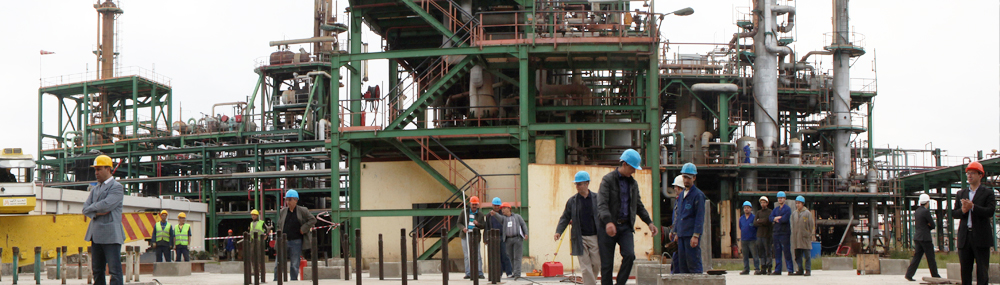
\includegraphics[width=12cm]{images/couvert.jpg}
			\label{fig:figure}
		\end{center}
	\end{figure}

\begin{minipage}{1\textwidth}												

\end{minipage}\\[2cm]
	
	
	\begin{minipage}{1\textwidth}												
		\begin{center}	 \large															
			\emph{Réalisé par:}\\[0.3cm]
			\textbf{ACHAQ Abdelkarim } \\
			\textbf{FILALI Ahmed } \\
		
		\end{center}																		
	\end{minipage}\\[3cm]
	
	
	%\bigskip{}
	\begin{minipage}{1\textwidth}												
		\begin{center}	 \large															
			
			%\includegraphics[scale = 0.6]{} \\
		\end{center}															
	\end{minipage}\\[0.5cm]
		\begin{minipage}{1\textwidth}												
					
	\end{minipage}\\[2cm]
	
	
	\begin{minipage}{1\textwidth}
	\begin{center} \large
		\emph{Encadré par :}\\[0.3cm]

		\centering	\item  \textbf{Mr. CHERKAOUI Mohammed} 
					
	\end{center}
	\end{minipage}\\[2.5cm]
	
\end{center}

\setcounter{page}{0}
\thispagestyle{empty}

\newpage
\newpage
\pagenumbering{roman}



%*********************************************Resume************************************************************
%*\chapter*{Résumé}
%*********************************************Abstract************************************************************
%\chapter*{Abstract}

\tableofcontents
\setcounter{tocdepth}{5}

\newpage
\listoffigures


\newpage
\sf
%-------------------------------------------------------------------------------------------------------------------
%************************************************Intoduction********************************************************
%-------------------------------------------------------------------------------------------------------------------
\chapter*{Introduction}
\addcontentsline{toc}{chapter}{\numberline{}Introduction}
Les bases de données sont aujourd’hui un élément omniprésent tant dans l’industrie que dans les
organismes publics. Grâce au développement exponentiel des outils informatiques de stockage et
aussi d’espace mémoire de plus en plus fiables, faciles à gérer et bon marché, les bases de données
deviennent chaque jour de plus en plus massives et complexes. Si on ajoute aussi que la
connaissance est une arme très importante en compétition, il devient évident qu’il faut disposer des
outils qui permettent de clarifier et obtenir avec précision et rapidité l’information utile résidant e
dans ces données, la plupart du temps caché à l’œil humain.Les entreprises sont confrontées à certaines problématiques qui sont celles de savoir comment
collecter, stocker, analyser et exploiter ces grands volumes de données pour créer de la valeur
ajoutée. C'est là qu'intervient les technologies d’analyse « Data Mining » et « Big Data », qui
englobe un ensemble de technologies et de pratiques destinées à stocker de très grandes masses de
données et à les analyser très rapidement.Les entreprises sont confrontées à certaines problématiques qui sont celles de savoir comment
collecter, stocker, analyser et exploiter ces grands volumes de données pour créer de la valeur
ajoutée. C'est là qu'intervient les technologies d’analyse « Data Mining » et « Big Data », qui
englobe un ensemble de technologies et de pratiques destinées à stocker de très grandes masses de
données et à les analyser très rapidement.

C'est dans cette optique que la Société Nationale d'electrolyse et de pytrochimie a décidé
de prendre en charge un projet d’analyse Data Mining et Big Data qui consiste à réaliser des
plateformes d’analyse Data Mining, intelligence artificielle et machine learning permettant de traiter et analyser les données et les experiences deja effectués du compound afin d’établir des statistiques descriptives et prédire une optimisation efficace en terme du temps en remplaçant l'ancienne methode de trial-errors.
%-------------------------------------------------------------------------------------------------------------------
%
%**************************************General Context****************************************************
%
%-------------------------------------------------------------------------------------------------------------------
\pagenumbering{arabic}


\chapter{CONTEXTE GENERALE DU PROJET}
\section*{problematique}
La Société Nationale d'Electrolyse et de Pétrochimie (SNEP) produit et commercialise une gamme de produits stratégiques et indispensables à l’activité de plusieurs secteurs industriels. Filiale de Ynna Holding, SNEP est le leader sur le marché Marocain des produits vinyliques (PVC et Compound PVC) et des produits issus de l'électrolyse (Soude, Chlore, Eau de Javel) et de l'Acide Chlorhydrique. 

Aujourd'hui, Le service du developpement présente l’un des principaux composants du département Compound. La maîtrise de son évolution constitue un objectif fort. En effet, pour bien accomplir sa mission, il est devenu indispensable que le service ait un processus d’analyse et de
traitement de la volumétrie des données recueillies depuis les anciennes experiences realisés

En effet ; la SNEP essaye de concevoir et de développer des produits et solutions
à la pointe du progrès, immédiatement adaptés aux dernières évolutions technologiques.


Donc on doit utiliser des outils technologiques avancées qui permettent de gérer ces données sans perdre leur valeur ajoutée et qui facilitent leur exploration afin d’améliorer et proposer un systeme capable de predire les quantités des additives necessaires pour obtenir les caracteristiques souhaités selon le compound ciblé avec un coùt efficace.
\begin{figure}[H]
	\begin{center}
		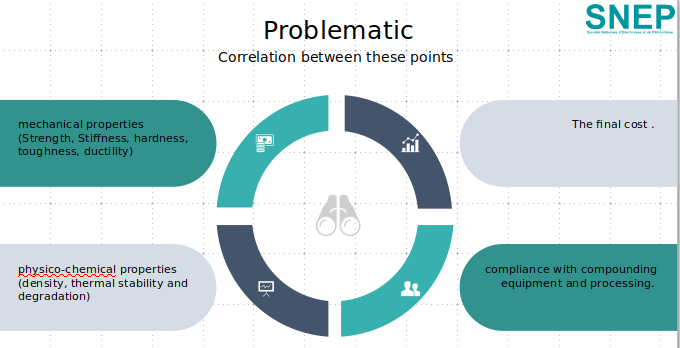
\includegraphics[width=12cm]{images/prob.png}
		\caption{la problematique}
		\label{fig:figure}
	\end{center}
\end{figure}


\paragraph{Donc comment peut-on résoudre cette problématique ?\\
Et Quelle technologie d’analyse des données sera convenable pour ce type de problématique ?
}
\section*{Solution}

\begin{figure}[H]
	\begin{center}
		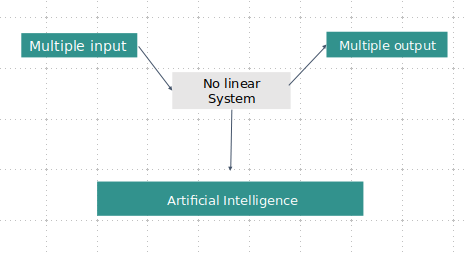
\includegraphics[width=12cm]{images/solutions.png}
		\caption{la solution introduit}
		\label{fig:figure}
	\end{center}
\end{figure}


\chapter{CONDUITE DU PROJET}
\section{Introduction}
La gestion du projet (ou conduite du projet) est une démarche visant à organiser de bout en bout
le bon déroulement du projet. Il est indispensable pour assurer une bonne gestion des moyens à
disposition (temps, information et ressources) afin de produire un système de bonne qualité tout en
optimisant les ressources disponibles. Pour réaliser un projet informatique, deux grandes familles de
méthodes existantes : l’approche classique avec le fameux cycle en V et l’approche agile avec des
méthodes comme « SCRUM ». Chacune de ces méthodes présente des avantages et des
inconvénients qu’il faut connaître pour faire le choix le plus pertinent pour la réussite du projet.
Dans ce chapitre, nous allons donner une vision sur la méthodologie choisie pour la réalisation
du projet ainsi que la planification de sa mise en œuvre.

\section{la methode agile}
Le terme "agile" définit une approche de gestion de projet qui prend le contre-pied des
approches traditionnelles prédictives et séquentielles de type cycle en V ou waterfall (en cascade).
La notion même de "gestion de projet" est remise en question au profit de "gestion de produit". De
façon à raisonner d’avantage "produit" que "projet". Après tout l'objectif d'un projet consiste bien à
donner naissance à un produit.
Une approche dite "traditionnelle" attend généralement du client une expression détaillée et
validée du besoin en entrée de réalisation, laissant peu de place au changement. La réalisation dure
le temps qu'il faut et le rendez-vous est repris avec le client pour la recette. Cet effet tunnel peut être
très néfaste et conflictuel, on constate souvent un déphasage entre le besoin initial et l'application
réalisée. On se rapporte alors aux spécifications validées et au contrat.
Certains projets se terminent dans la douleur (surtout dans le cadre d'un contrat au
forfait classique) au risque de compromettre la relation client. De plus il n'est pas rare que certaines
fonctionnalités demandées se révèlent finalement inutiles à l'usage alors que d'autres, découvertes en
cours de route, auraient pu donner plus de valeur au produit.
L'approche Agile propose au contraire de réduire considérablement voire complètement cet effet
tunnel en donnant d’avantage de visibilité, en impliquant le client du début à la fin du projet et en
adoptant un processus itératif et incrémental. Elle considère que le besoin ne peut être figé et
propose au contraire de s'adapter aux changements de ce dernier. Mais pas sans un minimum de
règles. Ce procédé est rapidement devenu populaire car il permet d’aligner le développement d’un
projet avec les besoins du client.\\
De plus, il correspond directement aux concepts du Manifeste Agile et est donc facile à mettre
en place. Ce manifeste a été écrit par quatorze leaders de l'industrie de l’édition logiciel qui ont créé
un processus basé sur leurs succès et leurs échecs passés.
La méthode Agile souscrit à un ensemble de rôles qui comprend :\\
+ Le responsable du projet, qui représente le client et clarifie les exigences avec l'équipe.\\
+ Le chef de projet, responsable de l'équipe.\\
+ L'équipe projet, qui constitue le groupe qui exécute le projet.\\
+ Les parties prenantes, étant toute personne ayant un intérêt dans le projet.

\section{la plannification du projet }
La planification est parmi les phases d'avant-projet. Elle consiste non seulement à délimiter le
périmètre temporel du projet, mais aussi à prévoir le déroulement des activités tout au long de la
période allouée au stage.
Généralement pour planifier un projet, la première phase consiste à le découper en plusieurs
étapes, d'en estimer la durée, d'identifier enchaînement des étapes (dont celles qui peuvent être
conduites en parallèle), affecter des ressources (financières et humaines), et enfin modéliser cette
organisation sur un document opérationnel partagé entre tous les acteurs concernés.
\\
\begin{figure}[H]
	\begin{center}
		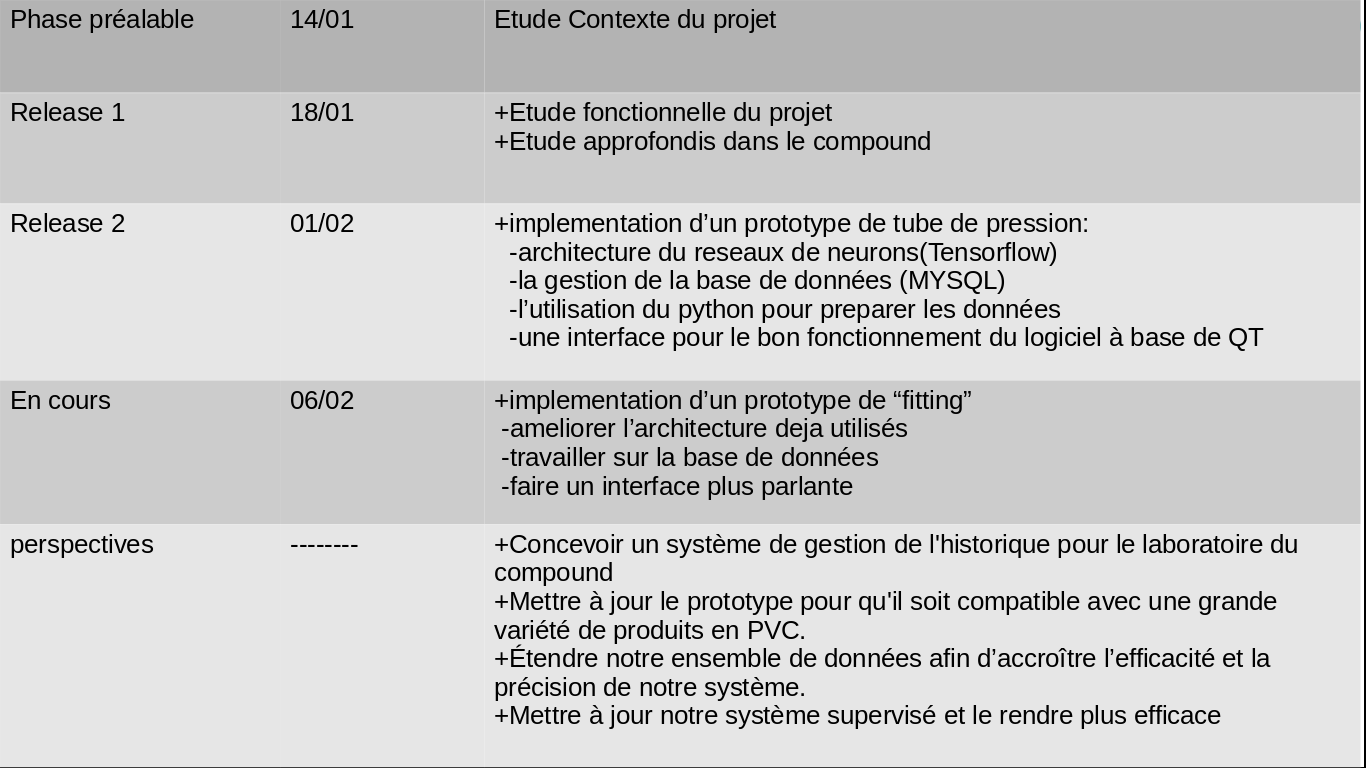
\includegraphics[width=15cm]{images/agile.png}
		\caption{le planning de notre projet}
		\label{fig:figure}
	\end{center}
\end{figure}


\chapter{technologies et methodologies}

\section{Machine learining}
\subsection{definition}
Même s’il est actuellement dopé par les nouvelles technologies et de nouveaux usages, le
machine learning n’est pas un domaine d’étude récent. On en trouve une première
définition dès 1959, due à Arthur Samuel, l’un des pionniers de l’intelligence artificielle,
qui définit le machine learning comme le champ d’étude visant à donner la capacité à une
machine d’apprendre sans être explicitement programmée. En 1997, Tom Mitchell, de
l’université de Carnegie Mellon, propose une définition plus précise :
« A computer program is said to learn from experience E with respect to some class of
tasks T and performance measure P, if its performance at tasks in T, as measured by P,
improves with experience E ».
\begin{figure}[H]
	\begin{center}
		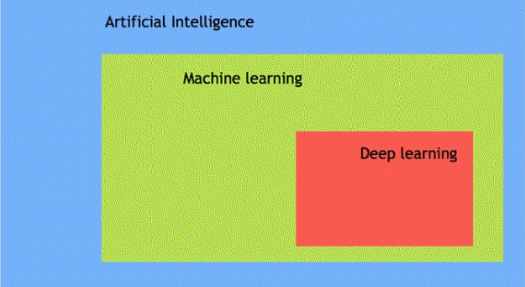
\includegraphics[width=12cm]{images/artint.png}
		\caption{La difference entre : intelligence artificielle-machine learning-deep learning)}
		\label{fig:figure}
	\end{center}
\end{figure}

Un robot qui apprend à conduire ? Cela peut paraître un peu loin de vos préoccupations…
mais illustrons brièvement ce que peut faire le machine learning avec un cas simple, sans
doute plus proche de votre quotidien : un filtre antispam. Dans un premier temps, on peut
imaginer que la « machine » (votre service de messagerie) va « analyser » la façon dont
vous allez classer vos mails entrants en spam ou pas. Grâce à cette période
d’« apprentissage », la machine va déduire quelques grands critères de classification. Par
exemple, la probabilité que la machine classe un mail en spam va augmenter si le mail
contient des termes tels qu’« argent », « rencontre facile » ou « viagra » et si l’expéditeur
du mail n’est pas dans votre carnet d’adresses. A contrario, la probabilité de classement en
spam va baisser si l’expéditeur est connu et que les mots du mail sont plus « classiques ».
On laissera le lecteur choisir la définition du machine learning avec laquelle il est à l’aise.
Le tout est de bien comprendre la métaphore de l’apprentissage de la machine (à opposer à
une programmation impérative de type règle « IF… THEN… ELSE… »), qui permettra à
la machine d’apprendre à partir de données réelles. Avec le machine learning, on passe
d’une informatique impérative basée sur des hypothèses à une informatique probabiliste
basée sur des informations réelles. Mais pour se lancer dans cette aventure, il nous faut
avant tout des données !\\
La data science est une démarche empirique qui se base sur des données pour apporter une
réponse à des problèmes. Donc, avant toute chose, assurez-vous d’avoir des données.\\

\subsection{type de données}
On distingue généralement les données quantitatives des données qualitatives.\\
Les données quantitatives sont des valeurs qui décrivent une quantité mesurable, sous la
forme de nombres sur lesquels on peut faire des calculs (moyenne, etc.) et des
comparaisons (égalité/différence, infériorité/supériorité, etc.). Elles répondent typiquement
à des questions du type « combien ». On fait parfois la différence entre :\\
• les données quantitatives continues, qui peuvent prendre n’importe quelle valeur dans un
ensemble de valeurs : la température, le PIB, le taux de chômage, en sont des exemples ;\\
• et les données quantitatives discrètes, qui ne peuvent prendre qu’un nombre limité de
valeurs dans un ensemble de valeurs : le nombre d’enfants par famille, le nombre de
pièces d’un logement, etc.
Les données qualitatives décrivent quant à elles des qualités ou des caractéristiques. Elles
répondent à des questions de la forme « quel type » ou « quelle catégorie ». Ces valeurs ne
sont plus des nombres, mais un ensemble de modalités. On ne peut pas faire de calcul sur
ces valeurs, même dans l’éventualité où elles prendraient l’apparence d’une série
numérique. Elles peuvent toutefois être comparées entre elles et éventuellement triées. On
distingue :\\
• les données qualitatives nominales (ou catégorielles), dont les modalités ne peuvent être
ordonnées. Par exemple : la couleur des yeux (bleu, vert, marron, etc.), le sexe (homme,
femme), la région d’appartenance (68, 38, etc.) ;\\
• et les données qualitatives ordinales, dont les modalités sont ordonnées selon un ordre
« logique ». Par exemple : les tailles de vêtements (S, M, L, XL), le degré d’accord à un
test d’opinion (fortement d’accord, d’accord, pas d’accord, fortement pas d’accord).
\begin{figure}[H]
	\begin{center}
		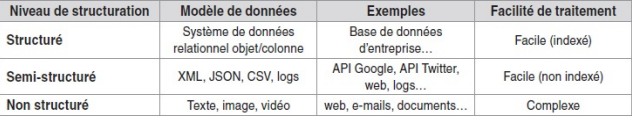
\includegraphics[width=12cm]{images/data_type.png}
		\caption{les types des données}
		\label{fig:figure}
	\end{center}
\end{figure}

\subsection{les algorithmes}
Quel que soit l’algorithme qu’il utilise, le data scientist n’a qu’une seule idée en tête :
découvrir des liens dans ses données (on parle souvent de pattern). Dans le cadre de
l’emploi de méthodes de machine learning, on suppose donc qu’il existe un lien au sein
des données et que nos algorithmes vont nous aider à le trouver.\\
Les algorithmes ne sont pas tous destinés aux mêmes usages. On les classe usuellement
selon deux composantes
5
:
• le mode d’apprentissage : on distingue les algorithmes supervisés des algorithmes non
supervisés ;
• le type de problème à traiter : on distingue les algorithmes de régression de ceux de
classification.
\begin{figure}[H]
	\begin{center}
		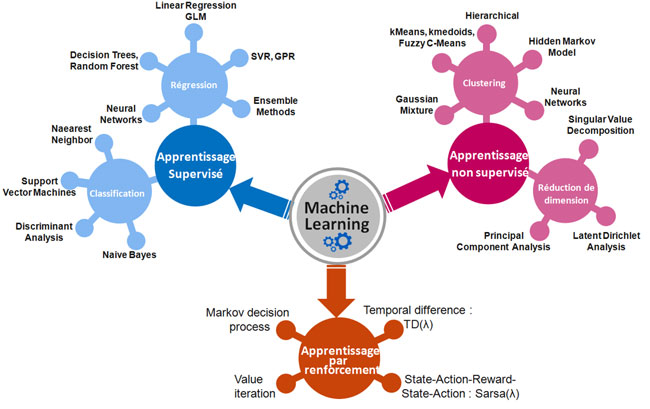
\includegraphics[width=12cm]{images/machine.jpg}
		\caption{type de machine learning}
		\label{fig:figure}
	\end{center}
\end{figure}
\subsubsection{Algorithmes supervisés et non supervisés}
La différence entre algorithmes supervisés et non supervisés est fondamentale. Les
algorithmes supervisés extraient de la connaissance à partir d’un ensemble de données
contenant des couples entrée-sortie. Ces couples sont déjà « connus », dans le sens où les
sorties sont définies a priori. La valeur de sortie peut être une indication fournie par un
expert : par exemple, des valeurs de vérité de type OUI/NON ou MALADE/SAIN. Ces
algorithmes cherchent à définir une représentation compacte des associations entrée-sortie,
par l’intermédiaire d’une fonction de prédiction.\\
Au contraire , les algorithmes non supervisés n’intègrent pas la notion d’entrée-sortie.
Toutes les données sont équivalentes (on pourrait dire qu’il n’y a que des entrées). Dans ce
cas, les algorithmes cherchent à organiser les données en groupes. Chaque groupe doit
comprendre des données similaires et les données différentes doivent se retrouver dans des
groupes distincts. Dans ce cas, l’apprentissage ne se fait plus à partir d’une indication qui

peut être préalablement fournie par un expert, mais uniquement à partir des fluctuations
observables dans les données.\\
Le petit exemple qui suit illustre les principes de ces deux familles d’algorithmes.
Imaginons un ensemble d’individus décrits par deux variables d’entrée, X1 et X2
.
 Dans le cas d’un apprentissage supervisé, il faudra leur adjoindre une variable de sortie Y, qui
pourra par exemple prendre deux valeurs {O, X}. L’algorithme proposera alors une
fonction de prédiction de la forme Y = f(X1
, X2
). Dans le cas de l’apprentissage non
supervisé, plus de Y : l’algorithme va trouver tout seul, comme un grand, deux groupes
d’individus distincts, juste à partir des positions dans le plan défini par X1 et X2
, et ce sans
aucune autre indication. 

\begin{figure}[H]
	\begin{center}
		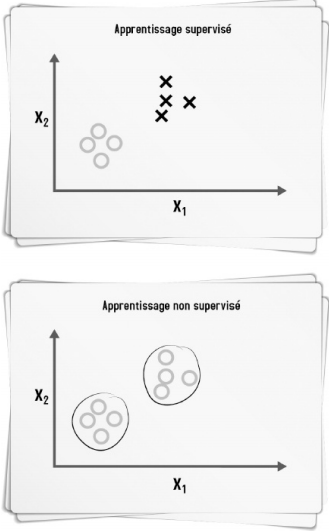
\includegraphics[width=12cm]{images/supervised.png}
		\caption{ Apprentissages supervisé et non supervisé}
		\label{fig:figure}
	\end{center}
\end{figure}

\paragraph{dans notre cas , et puisque on cherche à predire les additives necessaire pour certain caracteristiques ,il faut être capable de spécifier une valeur de sortie, et cette information d’expert n’est pas
	toujours disponible. dans ce cas les algorithmes supervisés sont plus performants}


\section{technologies de developpement }
\subsection{Python}
 est un langage de programmation objet interprété sous licence libre et fonctionne sur la plupart des plates-formes informatiques,c'est un langage qui peut s'utiliser dans de nombreux contextes et s'adapter à tout type d'utilisation grâce à des bibliothèques spécialisées Il est particulièrement répandu dans le monde scientifique, et possède de nombreuses bibliothèques optimisées destinées au calcul numérique, la raison pour laquelle on l'a choisi pour le déveleoppemrnt de notre application.
 \begin{figure}[H]
 	\begin{center}
 		
\includegraphics[width=4cm]{images/python.png}
 		\label{fig:figure}
 	\end{center}
 \end{figure}
 
 \subsection{TensorFlow}
 est un outil open source d'apprentissage automatique développé par Google,il s'agit de l'un des outils les plus utilisés en intelligence artificielle dans le domaine de l'apprentissage machine. Caractérisé par la richesse de bibliothèques qui permettent la bonne manipulation et gestion des réseaux de neurones ce qui le rend l'outil adéquat à notre projet.
  \begin{figure}[H]
 	\begin{center}
 		
\includegraphics[width=4cm]{images/tensor.png}
 		\label{fig:figure}
 	\end{center}
 \end{figure}
 
 \subsection{Mysql}
 est un système de gestion de bases de données relationnelles. Il fait partie des logiciels de gestion de base de données les plus utilisés au monde, autant par le grand public (applications web principalement) que par des professionnels, c'est l'outil qui va nous permettre de construire, alimenter, gérer puis communiquer avec notre base de données.
  \begin{figure}[H]
 	\begin{center}
 		
\includegraphics[width=4cm]{images/mysql.png}
 		\label{fig:figure}
 	\end{center}
 \end{figure}
 
 \subsection{QT}

(prononcé officiellement en anglais cute) un framework pour concevoir des interfaces graphiques, sa compatibilté avec le langage Python et son ergonomie nous a poussé de le choisir comme outil d'interfaçage homme machine.


 \begin{figure}[H]
	\begin{center}
		
\includegraphics[width=4cm]{images/qt.png}
		\label{fig:figure}
	\end{center}
\end{figure}

\chapter{Implementation du prototype tube de pression}

\section{preparation des données}

La base de données est le pilier du domaine de l'intelligence artificielle, donc cette dèrnieres doit répondre à des critères, en occurence, la richesse(on parle des milliers d'échantillons) ainsi que la divérsité des cas possibles.

Voici à quoi ressemblera une base de données qui sérvira par la suite à l'entrainement de notre système.
pour preparerla base de données , on s'est appuié sur les intervales données par Mr. Cherkaoui , et les données qu'on trouvé dans le laboratoire comme suit : 

\begin{figure}[H]
	\begin{center}
		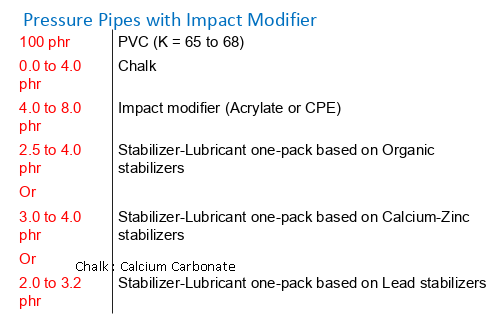
\includegraphics[width=12cm]{images/intervale.png}
		\caption{l'intervale des ingredients}
		\label{fig:figure}
	\end{center}
\end{figure}

et voici le resultat :
\begin{figure}[H]
	\begin{center}
		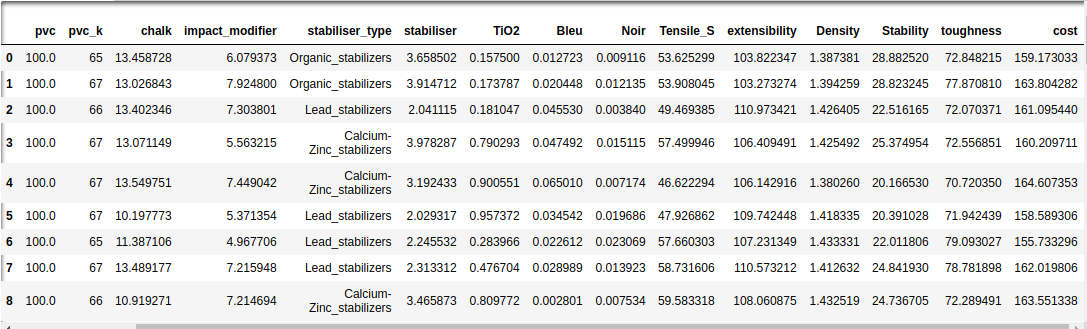
\includegraphics[width=12cm]{images/data.png}
		\caption{la preparation de la base de données}
		\label{fig:figure}
	\end{center}
\end{figure}


\section{la phase de training \& test}

Une fois que nous avons choisi l'architecture du réseau de neurones, c'est-à-dire le type de réseau de neurones, les fonctions d'activation, etc..., nous devons déterminer les autres paramètres ajustables du modèle que sont les poids qui permettent de connecter les entrées aux neurones cachées et les neurones cachés aux neurones de sortie. Le processus d'ajustement de ces paramètres de telle sorte que le réseau soit en mesure d'approcher la relation fonctionnelle sous-jacente entre les entrées x et les cibles t est connu sous le nom d'apprentissage. C'est au cours de ce processus que le réseau de neurones va apprendre à modéliser les données par des exemples. Bien qu'il existe différentes manières de réaliser l'apprentissage des réseaux de neurones, la plupart d'entre elles utilisent des algorithmes numériques qui sont en mesure d'effectuer la tâche au cours d'un nombre fini d'itérations. Nous avons recours à ces algorithmes itératifs essentiellement en raison de la nature fortement non-linéaire des modèles de réseau de neurones pour lesquels une solution en forme fermée n'est généralement pas disponible. Un algorithme d'apprentissage itératif va ajuster graduellement les poids du réseau de neurones de telle sorte que pour toute donnée d'entrée x, le réseau de neurones est en mesure de produire une sortie aussi proche que possible de t.

\subsection{Initialisation des Poids}
Puisque l'apprentissage des réseaux de neurones fait appel à un algorithme itératif au cours duquel les poids sont ajustés, il faut tout d'abord initialiser les poids avec des valeurs de départ raisonnables. Car ce sont non seulement la qualité de la solution mais également le temps nécessaire pour préparer le réseau (apprentissage) qui sont en jeu. Il est important d'initialiser les poids en utilisant de petites valeurs pour les poids de sorte que, au début de l'apprentissage, le réseau fonctionne en mode linéaire, puis qu'il augmente les valeurs de ses poids afin d'ajuster les données avec suffisamment de précision.

STATISTICA Réseaux de Neurones Automatisés intègre deux méthodes aléatoires pour initialiser les poids en utilisant la distribution normale et la distribution uniforme. La méthode normale va initialiser les poids en utilisant des valeurs distribuées normalement, dans un intervalle dont la moyenne est égale à zéro et l'écart-type est égal à un. La méthode uniforme va quant à elle affecter les valeurs des poids dans un intervalle compris entre 0 et 1.

\subsection{Apprentissage du Réseau de Neurones - Apprentissage par les Exemples}
Un réseau de neurones n'est pas en mesure de faire des prévision s'il n'a pas été entraîné préalablement sur des exemples connus sous le nom de données d'apprentissage. Les données d'apprentissage sont généralement constituées de couples entrée-cible qui sont présentés au réseau les uns après les autres lors de la phase d'apprentissage afin d'apprendre. Vous pouvez considérer les instances des entrées comme des "questions" et les valeurs cible comme des "réponses". Ainsi, à chaque fois qu'un couple d'entrée-cible est présenté au réseau de neurones, ce dernier connaît la réponse pour une question donnée. Il n'en demeure pas moins qu'à chaque instance, le réseau de neurones doit faire une supposition à l'aide des valeurs actuelles des poids, et ses performances sont alors testées en utilisant un critère connu sous le nom de fonction d'erreur. Si la performance n'est pas adéquate, les poids du réseau sont alors ajustés afin de produire une réponse exacte (ou du moins, plus exacte) par rapport à la précédente tentative.
\\
Remarque : La performance de la régression se calcule dans SANN comme la corrélation entre la valeur de sortie et la valeur prévue. La performance de la classification dans SANN performance comme le pourcentage d'observations correctement classées.

\begin{figure}[H]
	\begin{center}
		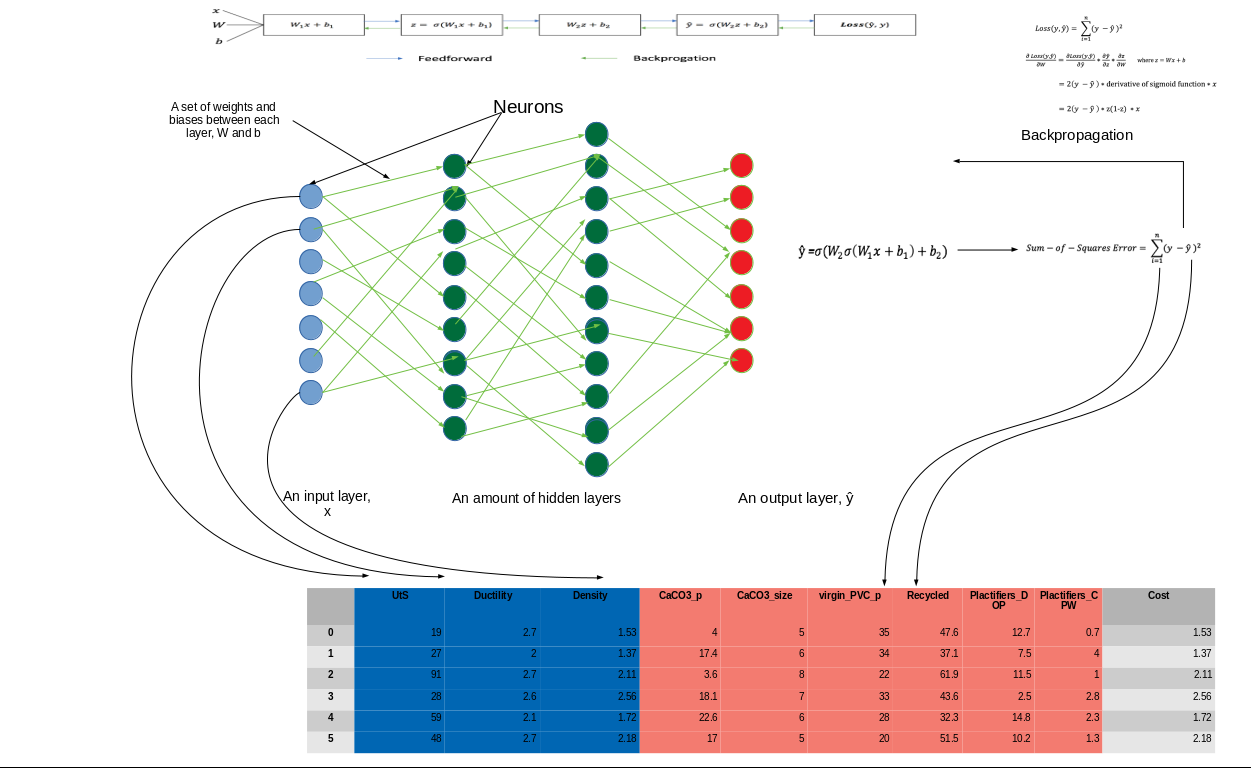
\includegraphics[width=12cm]{images/neural.png}
		\caption{le reseau de neurons utilisé}
		\label{fig:figure}
	\end{center}
\end{figure}
D'une manière générale, ce processus d'apprentissage intègre un certain bruitage (c'est-à-dire que les réponses du réseau peuvent être parfois plus exactes lors du cycle précédent de l'apprentissage par rapport au cycle actuel), mais en moyenne, l'importance des erreurs s'amenuise à mesure que l'apprentissage du réseau progresse. L'ajustement des poids s'effectue par le biais d'un algorithme d'apprentissage, qui comme un professeur, va apprendre au réseau de neurones à choisir ses poids afin d'obtenir de meilleures prévisions pour chacun des couples d'exemples entrée-cible du fichier de données.

Les étapes ci-dessus constituent l'apprentissage. Du point de vue des calculs, il repose sur la série d'étapes ci-dessous :
\\
Présenter au réseau un couple entrée-cible.
\\
Calculer les prévisions du réseau pour les cibles.
\\
Utiliser la fonction d'erreur pour calculer la différence entre les prévisions (sorties) du réseau et les valeurs cible. Reprendre les étapes 1 et 2 jusqu'à ce que tous les couples entrée-cible aient été présentés au réseau.
\\
Utiliser l'algorithme d'apprentissage afin d'ajuster les poids du réseau de telle sorte qu'il produise de meilleures prévisions à chaque couple entrée-cible. Remarque : les étapes 1 à 5 constituent un seul cycle d'apprentissage ou itération. Le nombre de cycles nécessaire pour entraîner un modèle de réseaux de neurones n'est pas connu a priori mais peut être défini dans le cadre du processus d'apprentissage.
\\
Répéter à nouveau les étapes 1 à 5 pendant un certain nombre de cycles d'apprentissage ou d'itérations jusqu'à ce que le réseau commence à produire des résultats suffisamment fiables (c'est-à-dire des sorties qui se trouvent assez proches des cibles compte tenu des valeurs d'entrée). Une processus d'apprentissage type pour les réseaux de neurones est constitué de plusieurs centaines de cycles.
\subsection{La Fonction d'Erreur}


Comme indiqué précédemment, la fonction d'erreur permet d'évaluer la performance d'un réseau de neurones au cours de l'apprentissage. Vous pouvez considérer qu'il s'agit d'un examinateur qui évalue les performances d'un étudiant. La fonction d'erreur indique dans quelle mesure les prévisions du réseau sont proches des valeurs cible et donc, quel ajustement doit être apporté aux poids par l'algorithme d'apprentissage à chaque itération. La fonction d'erreur représente donc d'une certaine manière les yeux et les oreilles de l'algorithme d'apprentissage pour savoir si le réseau est performant ou non compte tenu de l'état actuel de l'apprentissage (et donc, quel ajustement doit être apporté aux valeurs de ses poids).

Toutes les fonctions d'erreur utilisées pour l'apprentissage des réseaux de neurones doivent intégrer une certaine mesure des distances entre les valeurs cible et les prévisions correspondant aux entrées. Une approche courante consiste à utiliser la fonction d'erreur dite de somme des carrés. Dans ce cas, le réseau va apprendre une fonction discriminante. L'erreur de la somme des carrés est simplement donnée par la somme des différences entre les valeurs cibles et les sorties prévues définies pour l'ensemble d'apprentissage.

qui considère que les variables cible suivent une distribution multinomiale. Au contraire, l'erreur de la somme des carrés va modéliser la distribution des valeurs cible comme une fonction de densité de probabilités normale.

\section{interface QT pour la prediction}
\begin{figure}[H]
	\begin{center}
		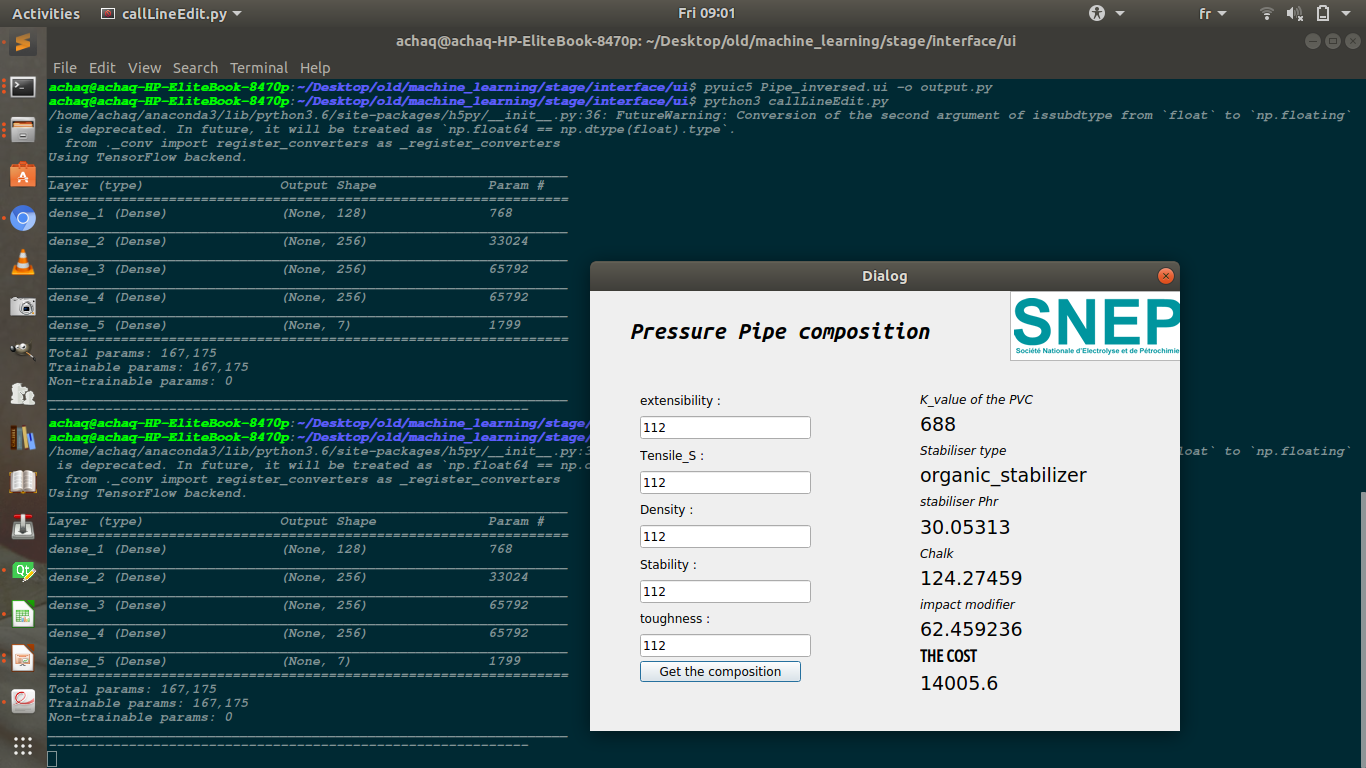
\includegraphics[width=12cm]{images/implement.png}
		\caption{l'interface à base de QT}
		\label{fig:figure}
	\end{center}
\end{figure}


\chapter*{Perspectives}
\addcontentsline{toc}{chapter}{\numberline{}Conclusion}

\paragraph{Concevoir un système de gestion de l'historique pour le laboratoire du compound\\
Mettre à jour le prototype pour qu'il soit compatible avec une grande variété de produits en PVC.\\
Étendre notre ensemble de données afin d’accroître l’efficacité et la précision de notre système.\\
Mettre à jour notre système supervisé et le rendre plus efficace}





%-------------------------------------------------------------------------------------------------------------------
%
%**************************************** Bibliography *******************************************
%
%-------------------------------------------------------------------------------------------------------------------
\newpage

\bibliographystyle{alpha}	
\bibliography{sample}
\thispagestyle{empty}


[1][Titow W.V.] PVC Technology (4th ed.).

[2][Aurélien Géron] Hands-On Machine Learning with Tensorflow \& python

[3][Atul Tripathi] Practical machine learning cookbook
\newpage

\appendix

\end{document}
